\documentclass[convert = false, tikz]{standalone}
\usepackage[utf8]{inputenc}
\usepackage{tikz}
\usetikzlibrary{automata, positioning, arrows}
 
\usepackage{../../../../style_automata}
% arara: pdflatex
% arara: latexmk: { clean: partial }


\usepackage{../../../../style_automata}

\begin{document}
\tikzset{initial text={}}
\begin{tabular}{cc}
    a=$r_1$: & \hspace{3cm}
    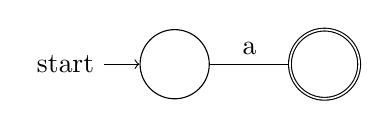
\begin{tikzpicture}[baseline=(current bounding box.center)]
        \node[state, initial] (s0) {};
        \node[state, accepting, right=of s0, node distance=3cm] (s1) {};
        
        \draw (s0) edge[above] node{a} (s1);
    \end{tikzpicture}
    \\
    b=$r_2$: & \hspace{3cm}
    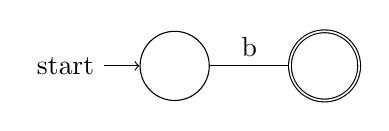
\begin{tikzpicture}[baseline=(current bounding box.center)]
        \node[state, initial] (s0) {};
        \node[state, accepting, right=of s0, node distance=3cm] (s1) {};
    
        \draw (s0) edge[above] node{b} (s1);
    \end{tikzpicture}
\end{tabular}
\end{document}
